\documentclass[../../main.tex]{subfiles}

\begin{document}
    
    Nach Einbau des Resonatormoduls (E) (siehe Kap. \ref{sec:Aufbau:Komponenten}) gemäß Kap. \ref{sec:Aufbau:NdYAGLaser} und Messung der Ausgangsleistung bei zwei gewählten Diodenlaserströmen $I_1 = 400\si{\mA}$ und $I_2 = 550\si{\mA}$ in Abhängigkeit von der Temperatur $T$ des Diodenlasers erhalten wir die Abbildungen \ref{fig:4:PowerOverTemperature_400mA_comp} und \ref{fig:4:PowerOverTemperature_550mA_comp}.

    % \begin{itemize}[label=$\to$]
    %     \item Welche Spiegeleigenschaft war gegeben? $R = 0.02$?
    % \end{itemize}

    \begin{figure}[H]
        \centering
        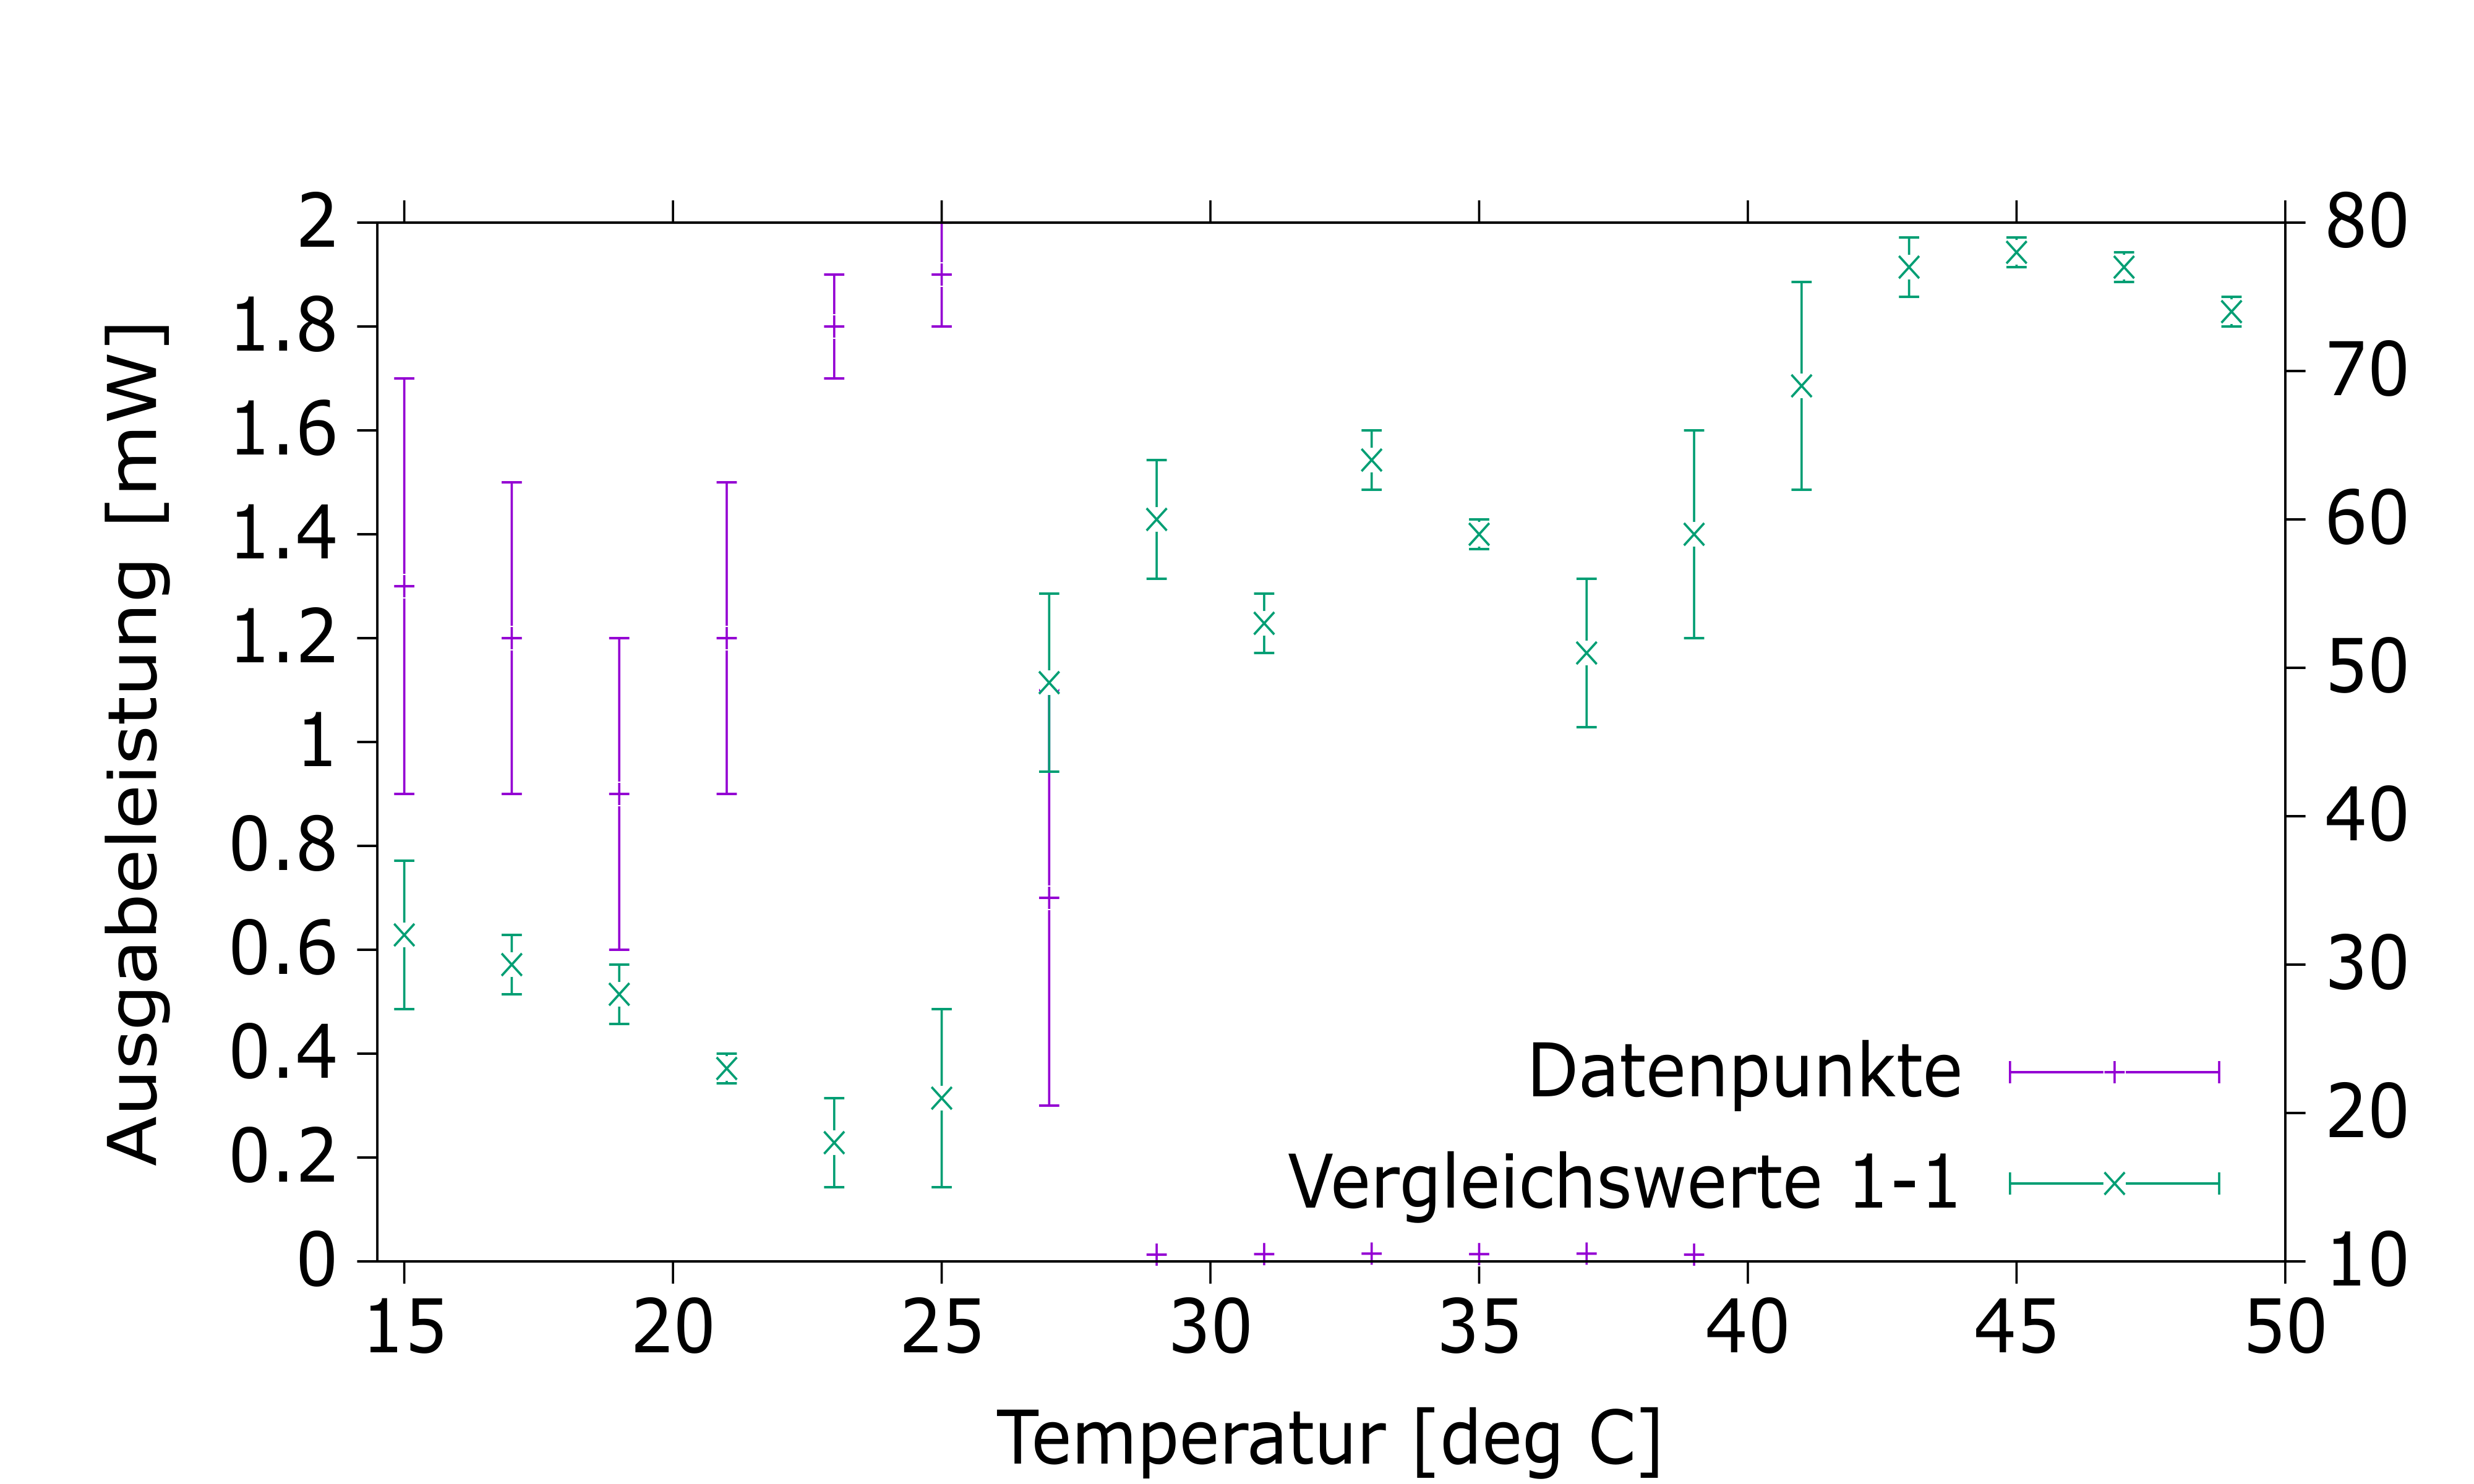
\includegraphics[width=11cm]{../../Bilddateien/4/PowerOverTemperature_400mA_comp.png}
        \caption{Die Ausgangsleistung des Nd:YAG Lasers als Funktion der Temperatur bei konstantem Anregungsstrom $I_{\textit{an}} = 400\si{\mA}$, verglichen mit dem Transmissionsspektrum des Nd:YAG Kristalls aus Kapitel \ref{subsec:1-1:Diodenlasertemperaturoptimierung}.}
    \end{figure}

    \begin{figure}[H]
        \centering
        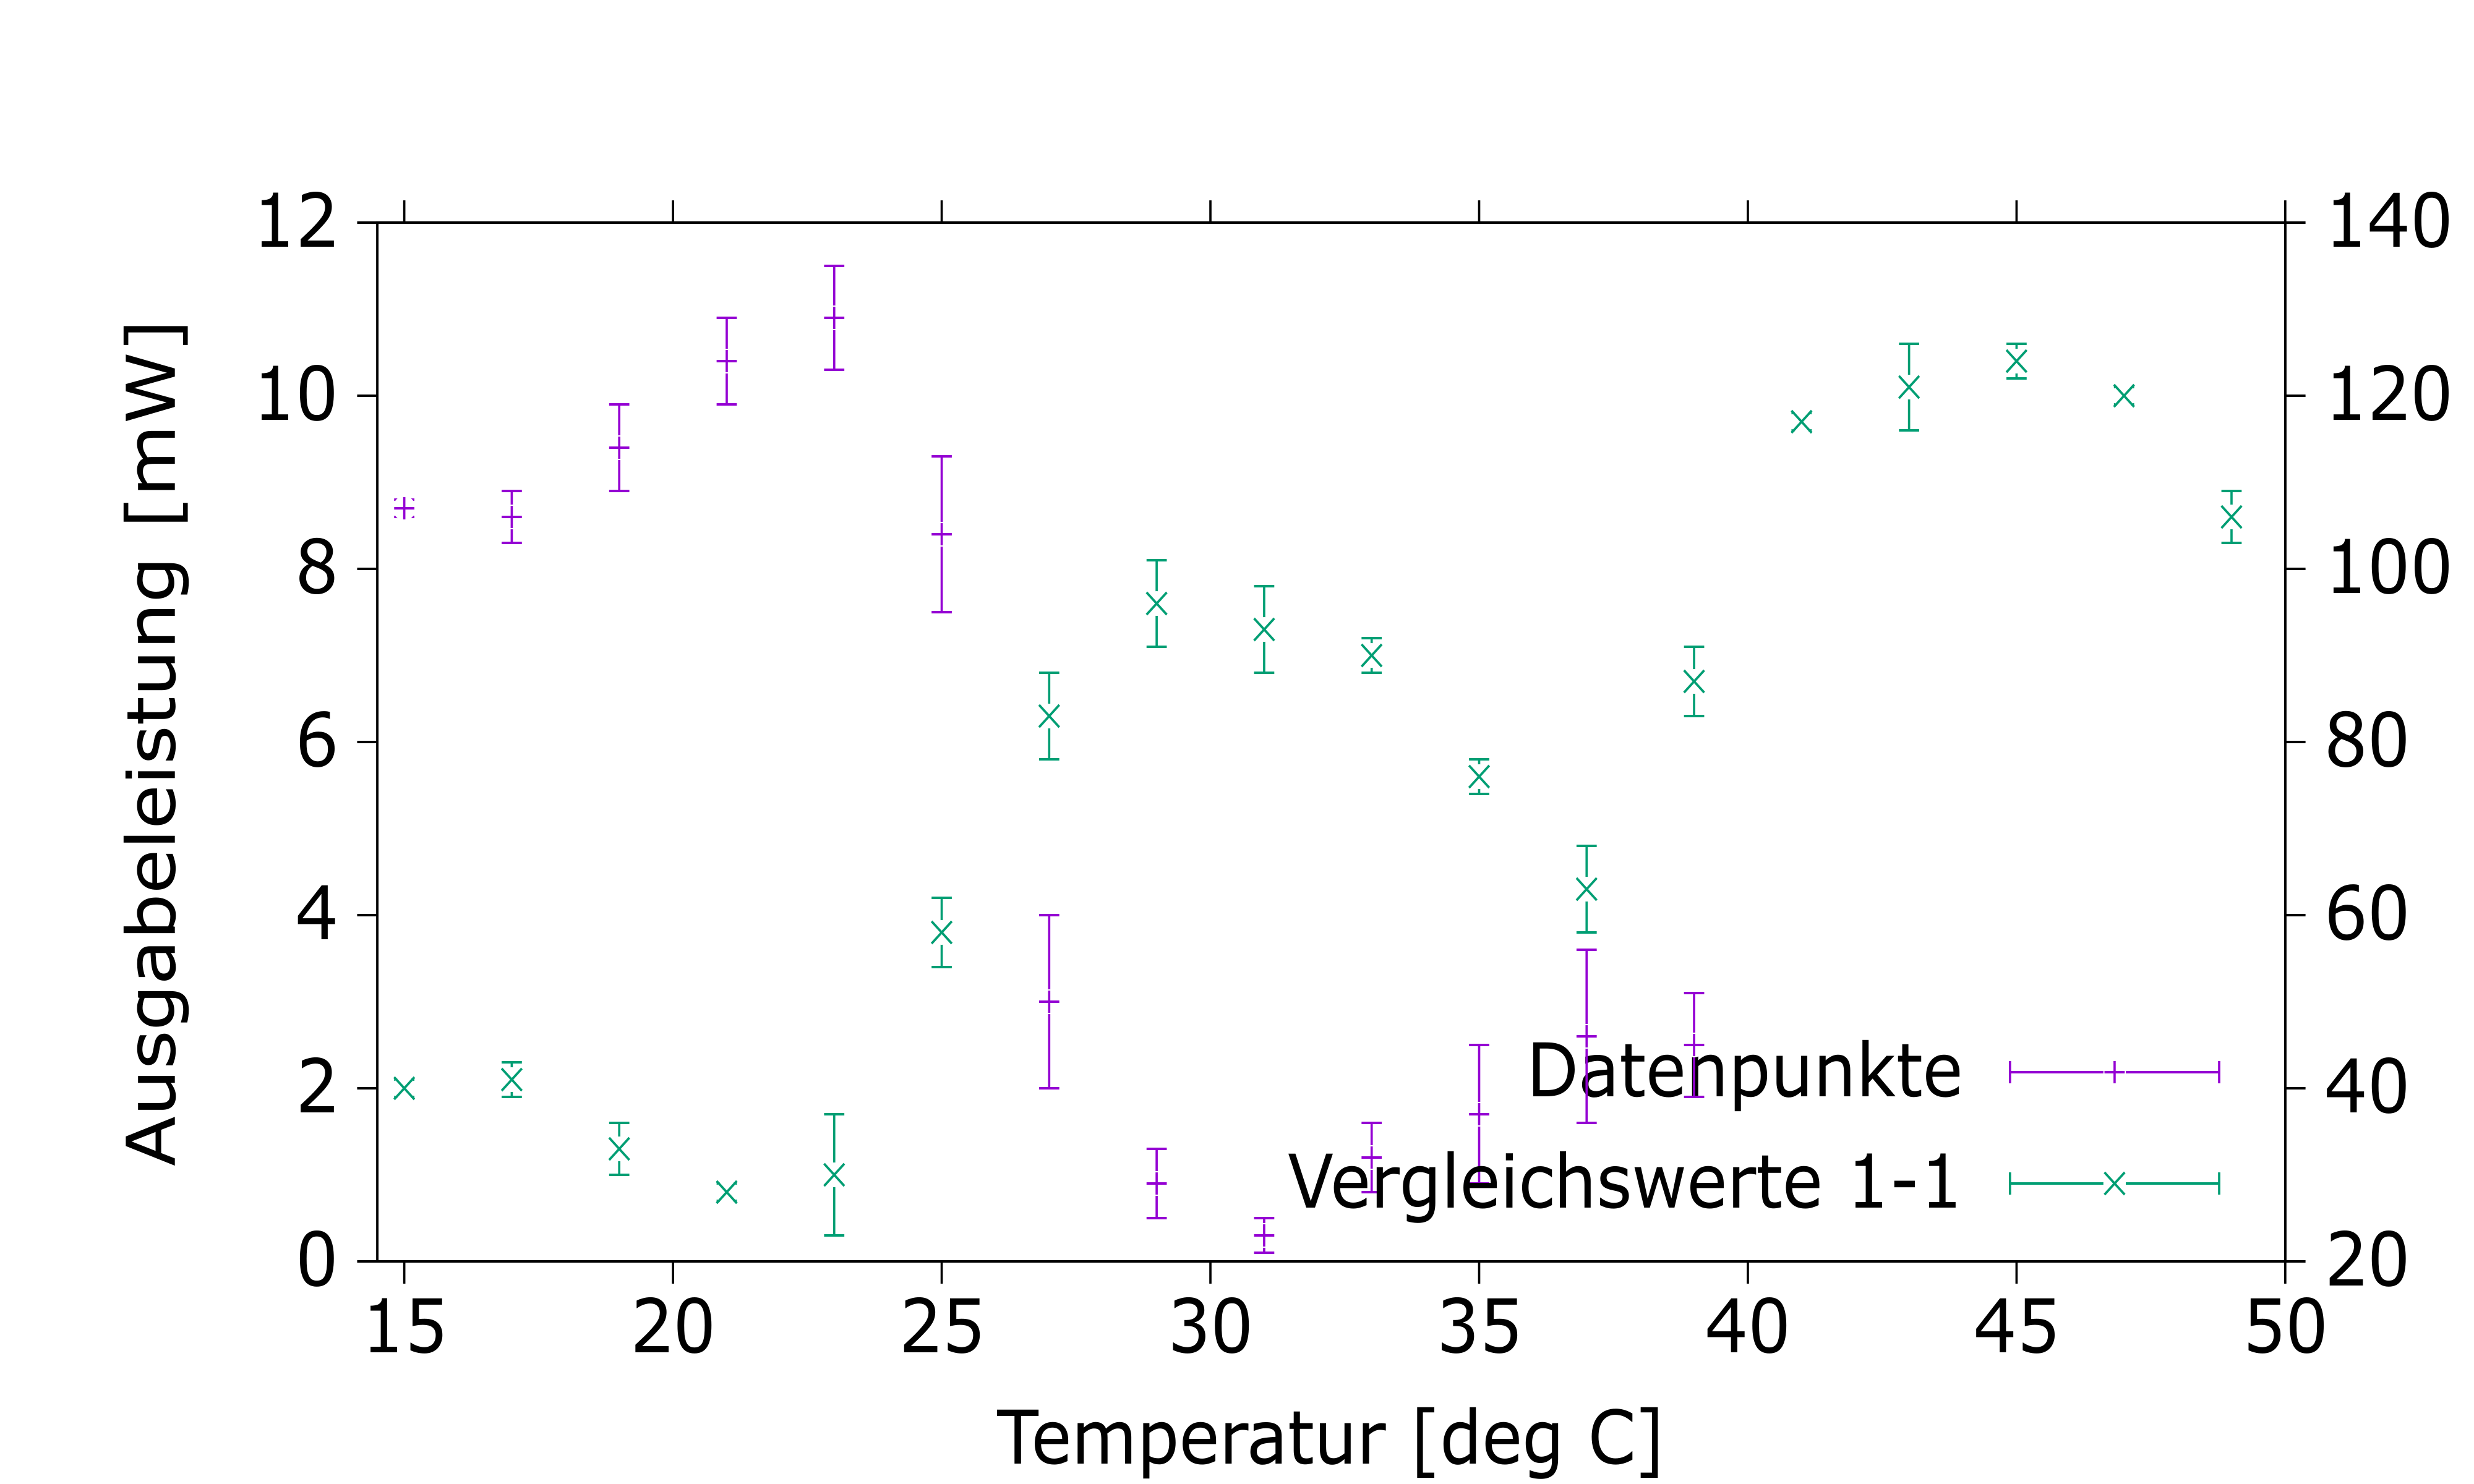
\includegraphics[width=11cm]{../../Bilddateien/4/PowerOverTemperature_550mA_comp.png}
        \caption{Die Ausgangsleistung des Nd:YAG Lasers als Funktion der Temperatur bei konstantem Anregungsstrom $I_{\textit{an}} = 550\si{\mA}$, verglichen mit dem Transmissionsspektrum des Nd:YAG Kristalls aus Kapitel \ref{subsec:1-1:Diodenlasertemperaturoptimierung}.}
    \end{figure}

    Durch den Vergleich mit dem in Kapitel \ref{subsec:1-1:Diodenlasertemperaturoptimierung} gemessenen Absorbtionsspektrum erkennen wir invertierte Optima: In Bereichen minimalen Durchsatzes des Absorbtionsspektrums erhalten wir beim Transmissionsspektrum maximale Werte. Hierbei ist jedoch die Skalierung der $y$-Achsen zu beachten, welche im Falle des Kristalls ohne Resonator deutlich niedriger (im Bereich $[0,2]$) ausfällt, während im Laserbetrieb die Ausgangsleistung zwischen $10\si{\mW}$ und $80\si{\mW}$ liegt.\\

\end{document}